\section{Rahmenpläne}\label{Rahmenplaene}
\begin{figure}[H]
    \centering
   \includegraphics[width=1\textwidth]{images/SoDa_Zeitstrahl_v1.png}
    \caption[SoDa Rahmenplan Version 1]{Rahmenplan Version 1,\\ Quelle: Autor}
    \label{img: SoDa Rahmenplan_v1}
\end{figure}
\section{Tokenauflösung mit jwt.io}\label{tokenaufloesung}
\begin{figure}[H]
	\centering
	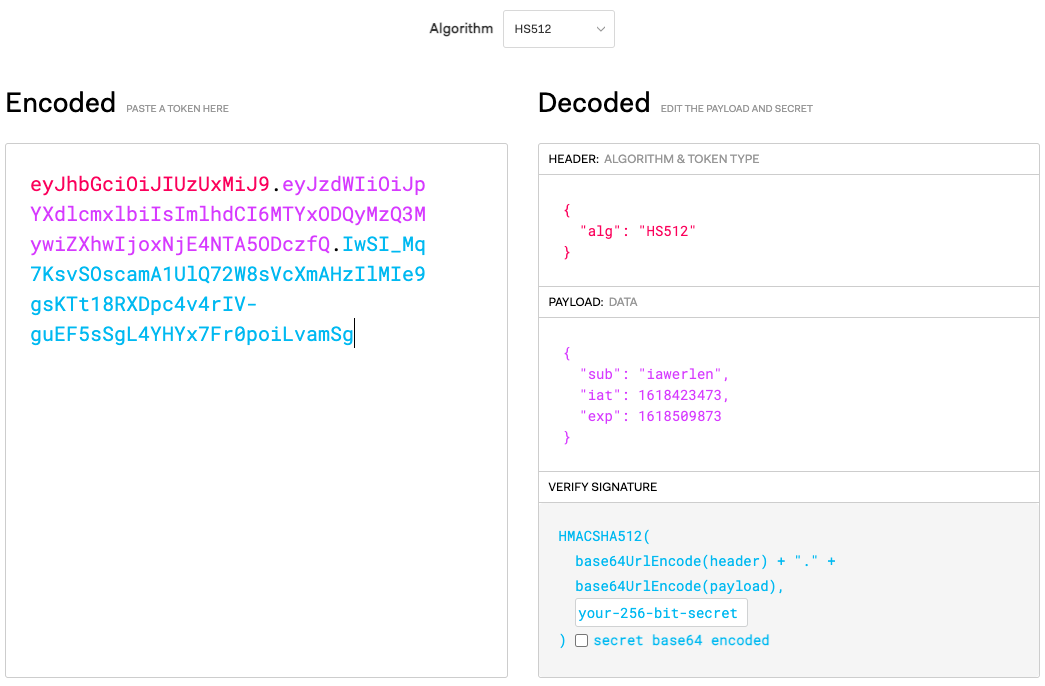
\includegraphics[scale=0.4]{images/jwtIO.PNG}
	\caption[Token Auflösung mit jwt.io]{Token Auflösung mit jwt.io, Quelle: Autor}
	\label{img: jwtio}
\end{figure} 
\section{Ausschnitt aus der Six Payment Backoffice}\label{sixPayment}
\begin{figure}[H]
	\centering
	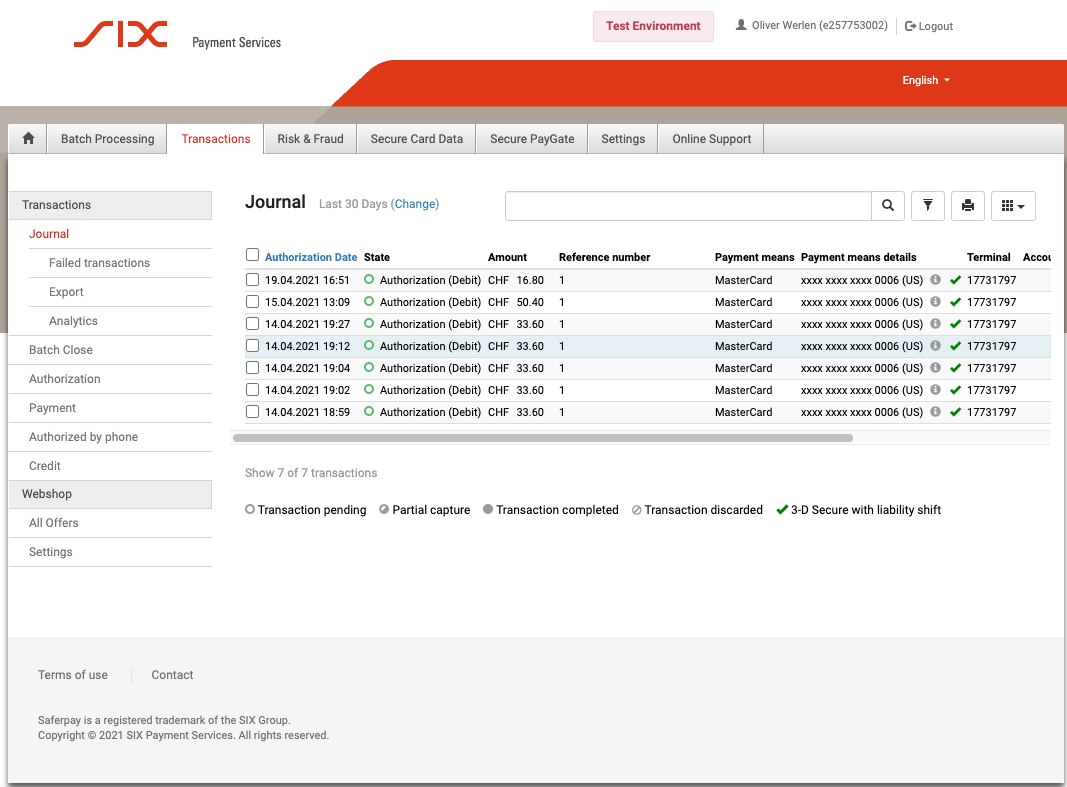
\includegraphics[width=1\textwidth]{images/paymentsBackoffice.PNG}
	\caption[Bezahlhistorie Backoffice]{Bezahlhistorie Backoffice, Quelle: Autor}
	\label{img: paymentsBackoffice}
\end{figure} 

\section{Drehbuch Pitching Video}
\subsection{Elevator Pitch}
Suchst auch du eine Möglichkeit, bequem mit deinem Smartphone Zigaretten zu kaufen und sie direkt abzuholen? 

\subsection{Problem}
Es gibt viele verschiedene Möglichkeiten, Tabakwaren zu kaufen- aber keine, die 24h verfügbar ist und auch vollkommen autonom.

\subsection{Lösung}
Die JTI Pick-Station ist die Lösung für dieses Problem. Sie ist 24h verfügbar, bietet einen schnellen, intuitiven Kaufprozess. Und das Beste: ohne Zusatzkosten.  

\subsection{Marktpotenzial}
27,1 Prozent der Schweizer Bevölkerung sind Raucher. 
Pro Tagen werden in Dagmarsellen 53 Millionen Zigaretten hergestellt. 

\subsection{Geschäftsmodell}
Preis pro Paket bleibt gleich
Mehr Kunden für JTI gewinnen
Finanzierung über Tabakverkauf

\subsection{Vergleich mit Wettbewerb}
Einfach und günstig im Aufbau (avec)
Weite Verbreitung von Stations (avec)
Keine Wartezeit, keine Lieferkosten (Coop at home) 
                                                                                                             
\subsection{Team}
Oliver Werlen, Informatik
Arnold Philipp, Elektrotechnik
Lucas Eberli, Maschinenbau

\subsection{Fazit}
enormes Marktpotenzial
einzigartig
innovativ
Kontaktdaten

\begin{figure}[H]
	\centering
	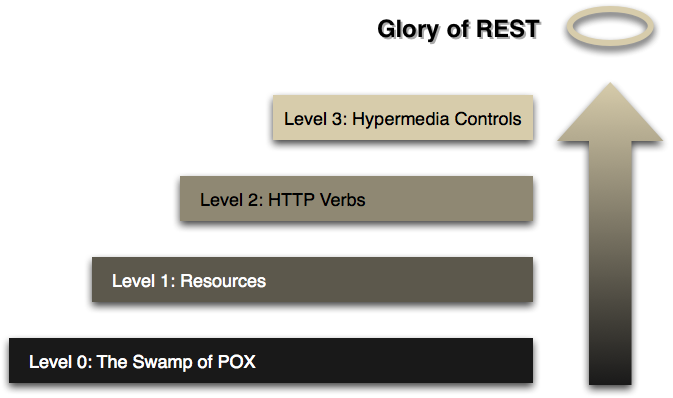
\includegraphics[scale=0.3]{images/richardsonMaturity.png}
	\caption[Richardson Maturity Model]{Richardson Maturity Model,\\ Quelle: \cite{richardsonMaturity}}
	\label{img: richardsonMaturity}
\end{figure}



